\documentclass[tikz]{standalone}
\usetikzlibrary{calc}

\begin{document}
    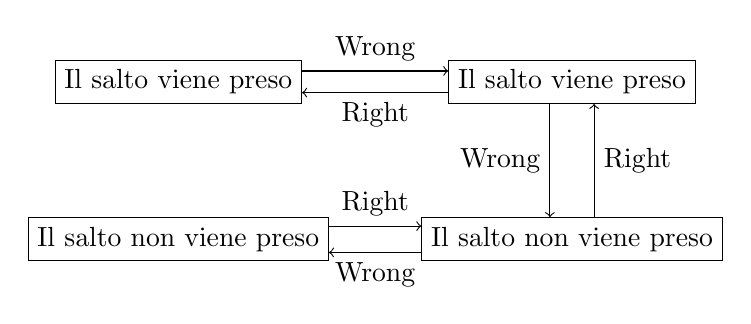
\begin{tikzpicture}
        \node[draw](suc0) at (0, 2) {Il salto viene preso};
        \node[draw](insuc0) at (0, 0) {Il salto non viene preso};
        \node[draw](suc1) at (5, 2) {Il salto viene preso};
        \node[draw](insuc1) at (5, 0) {Il salto non viene preso};

        \draw[->] (suc0.5) -- (suc1.175);
        \draw[->] (suc1.-175)-- (suc0.-5);
        \draw[->] (insuc0.5) -- (insuc1.175);
        \draw[->] (insuc1.-175)-- (insuc0.-5);
        \draw[->] (suc1.180+45) -- (insuc1.180-45);
        \draw[->] (insuc1.45) -- (suc1.-45);

        \node[above] at ($(suc0.5)!.5!(suc1.175)$) {Wrong};
        \node[below] at ($(suc0.-5)!.5!(suc1.-175)$) {Right};
        \node[above] at ($(insuc0.5)!.5!(insuc1.175)$) {Right};
        \node[below] at ($(insuc0.-5)!.5!(insuc1.-175)$) {Wrong};
        \node[left] at ($(suc1.180+45)!.5!(insuc1.180-45)$){Wrong};
        \node[right] at ($(insuc1.45)!.5!(suc1.-45)$){Right};
    \end{tikzpicture}
\end{document}
